\documentclass{article}

\usepackage{tikz} 

\usepackage{amsmath} % advanced math

% margins of 1 inch:
\setlength{\topmargin}{-.5in}
\setlength{\textheight}{9in}
\setlength{\oddsidemargin}{0in}
\setlength{\textwidth}{6.5in}

\usepackage{hyperref}
\hypersetup{
    colorlinks=true,
    linkcolor=blue,
    filecolor=magenta,      
    urlcolor=cyan,
    pdftitle={Overleaf Example},
    pdfpagemode=FullScreen,
    }
    
\usepackage{graphicx}
\graphicspath{ {./images/} }
\usepackage{float}
\usepackage[demo]{graphicx}
\usepackage{subfig}

\usepackage[english]{babel}
\usepackage[autostyle, english = american]{csquotes}
\MakeOuterQuote{"}

\begin{document}

    % https://stackoverflow.com/a/3408428/1164295
        \title{2022 Future Computing Summer Internship Project:\\(Creating examples of livelock for the Structural Simulation Toolkit Discrete Event Simulator)}
        \author{Melissa Jost\thanks{melissakjost@gmail.com}\ }
        \date{\today}
            \maketitle
        \begin{abstract}
            % This challenge problem was solved / progress was made
            The focus of this project is to remedy the lack of examples of various distributed system
            design problems, and our ability to detect these issues.  Our goal within this 
            repository was to use a simulation of \href{https://en.wikipedia.org/wiki/Deadlock#Livelock}{livelock} to come up with a set of metrics applicable to analyzing other systems.  More specifically, we simulated the 
            \href{https://en.wikipedia.org/wiki/Dining_philosophers_problem}{dining philosopher's scenario} within the \href{http://sst-simulator.org/}{Structural Simulation Toolkit (SST)}, and used different iterations of this problem to analyze if livelock had occurred.  
            While coming up with the simulation for this problem was relatively straight-forward, there is still more work 
            to be done in regards to solidifying and expanding on the metrics we chose to define this problem within distributed systems. We measured the state changes that each philosopher encountered, and measured the progress of the simulation based on these states to make a decision about whether or not our system was livelocked.
        \end{abstract}

\ \\
% see https://en.wikipedia.org/wiki/George_H._Heilmeier#Heilmeier's_Catechism

%\maketitle

\section{Project Description} % what problem is being addressed? 

% The challenge addressed by this work is ...
The challenge that is being addressed by this work is that while we have countless examples of 
what issues exist within distributed systems, as well as various ways to avoid them, there is 
still a lack of work that exists with regards to quantifying metrics to detect these issues.  
By creating these simulations, we provide concrete implementations of livelock, which can be 
helpful to both those working to better understand these issues, as well as those trying to 
understand how to use SST as a whole.


\section{Motivation} % Why does this work matter? Who cares? If you're successful, what difference does it make?

The users of this work include two main groups of people: those developing distributed systems, and those interested in learning how to use SST.  This work benefits people developing distributed systems by specifying a useful set of metrics for detecting these various design problems, 
even if in simple simulations, it could potentially save a lot of time in finding them in real systems in the future.  
For those learning SST, these simulations help give more, simple examples of how to use the toolkit.

\section{Prior work} % what does this build on?

When looking into current research on this topic, we found that there was a lack of information regarding the simulation of various distributed system problems, livelock included.  Livelock is closely related to \href{https://en.wikipedia.org/wiki/Deadlock}{deadlock}. There are more examples focused on deadlock than livelock.  Most papers that mentioned livelock either worked on creating a clear definition of what defined livelock, or noted what could be done to avoid the issue altogether.  From this, we mostly built off of other people's definitions of livelock to create metrics to detect it. \newline

One definition of livelock that stood out was Ho's paper which focused on the idea of ``forward progress.''\cite{a.ho}  The concept of forward progress is defined as "performing useful computation towards termination."  In this paper, the dining philosopher's scenario was also used to test their definition of livelock, in which they defined forward progress as the state in which any of the philosophers ate.  Both deadlock and livelock scenarios in this instance can be defined as the philosophers starving, which is how they detected a standstill in their system. \newline

Another definition of livelock by Fiedor's \cite{j.fiedor} builds on the idea of forward progress. They noted the previously discussed ideas of progress defining whether or not one was in livelock, or an infinite loop being an indication of livelock.  However, Fiedor writes that these elements on their own weren't enough.  Instead, they quantified their definition as being "detection of a looping behavior [and] also of the fact that this behavior could be escaped only if some of the livelocked threads could escape it."\cite{j.fiedor}  Essentially, loops and non-progress on their own could point to livelock, but could also be indicators of other behaviors, so it wasn't enough on its own. \newline

One last paper we looked at was one from North Caroline State University.\cite{k.tai}  This paper also focused on a defining livelock in regards to the progressmade in the simulation.  They pointed out that the code would be dependent on some "critical state", and whether or not we enter that state could point towards livelock in the simulation.  The difference between this paper and others is that their detection for livelock was presented in a clear algorithm, which was helpful for developing our own understanding of livelock. \newline

See \cite{texbook} for prior work in this area.

\section{How to do the thing}

% The software developed to respond to this challenge was run on (one laptop/a cluster of 100 nodes).
For the simulation, we are able to run it with one laptop, with a total of five philosophers.  This is how a 
majority of our analysis took place.  However, by including additional links and components, we could easily 
scale this simulation to model a bigger system.  In addition, in order to observe the philosophers in livelock, it is only necessary to have two philosophers within the simulation.  The benefit of having five philosophers is that other than this fitting the classic definition of the dining philosophers scenario, it allows us to observe partial-livelock within the system.  If you play around with the timings of the various philosophers, we can enter a scenario where, for example, only one of the philosophers is starved while everyone else gets to make progress in the simulation. \newline

The software is available \href{https://github.com/lpsmodsim/2022HPCSummer-Livelock}{here.}  To run the code, you need to run the Makefile.  An example of the output is shown below. In addition, more details on replicating the simulation are located in the \texttt{example.md} file within the repository.
 \begin{verbatim}
make
mkdir -p .build
singularity exec /usr/local/bin/additions.sif g++ -std=c++1y -D__STDC_FORMAT_MACROS -fPIC 
-DHAVE_CONFIG_H -I/opt/SST/11.1.0/include -MMD -c diningPhilosopher.cc 
-o .build/diningPhilosopher.o
mkdir -p .build
singularity exec /usr/local/bin/additions.sif g++ -std=c++1y -D__STDC_FORMAT_MACROS -fPIC 
-DHAVE_CONFIG_H -I/opt/SST/11.1.0/include -MMD -c diningTable.cc -o .build/diningTable.o
singularity exec /usr/local/bin/additions.sif g++ -std=c++1y -D__STDC_FORMAT_MACROS -fPIC 
-DHAVE_CONFIG_H -I/opt/SST/11.1.0/include -shared -fno-common -Wl,-undefined 
-Wl,dynamic_lookup -o liblivelock2.so .build/diningPhilosopher.o .build/diningTable.o
singularity exec /usr/local/bin/additions.sif sst-register livelock2 
livelock2_LIBDIR=/home/mkjost/projects/livelock/2022HPCSummer-Livelock/diningTableExample
singularity exec /usr/local/bin/additions.sif sst tests/diningPhilosopher.py 
...
Text output in output.txt
Simulation statistics in CSV files
Simulation is complete, simulated time: 150 Ks
 \end{verbatim}

\section{Models} % explanation of our SST model
Throughout the process of simulating the dining philosopher's problem, we were able to come up with a few different instances of the 
problem, as well as note down certain parameters that seemed to make livelock more or less likely to occur.  When looking into what components 
made the most sense to model, we had different iterations: one that focused on modeling philosopher components alongside a central dining table 
component, as well as philosophers alongside individual chopstick components.  This allowed us to explore the ways in which different simulations 
would potentially affect the likelihood, as well as the ways in which livelock would occur.  In addition, it also allowed us explore a more general simulation question of what made the most sense to model as components and links within SST.  From here, we set a list of parameters in our 
simulations to see what would induce livelock.  These parameters included:

\begin{itemize}
    \item \texttt{thinkingDuration}: The amount of time a philosopher spends thinking after placing down his chopsticks, whether that was after he finished eating, or while trying to allow another philosopher to eat
    \item \texttt{waitingDuration}: The frequency at which a philosopher checks the state of his hands, and sees whether or not he needs to place down his chopsticks to allow another philosopher to eat
    \item \texttt{eatingDuration}: The amount of time a philosopher spends holding both chopsticks when eating
    \item \texttt{randomseed}: This is a seed for our random number generator that randomizes our first pass at grabbing chopsticks
    \item \texttt{id}: This id allows the chopsticks or the dining table to be able to identify the philosopher
    \item \texttt{livelockCheck}: This indicates how many cycles we want to run our simulation for before exiting
    \item \texttt{windowSize}: This tells us how often we should check our system for potential livelock conditions
\end{itemize}

The most important parameters in this list are the \texttt{thinkingDuration} and the \texttt{waitingDuration}, because these set up two different sets of 
clocks within our simulation that run on different cycle lengths.  One cycle length is designated by \texttt{thinkingDuration}, and is where the 
philosopher sends requests to pick up chopsticks if necessary.  The other cycle length is designated by \texttt{waitingDuration}, which is what 
allows us to induce livelock.  Every time this clock cycle ticks, the philosopher checks the state of their hands, and if they’re only 
holding one chopstick, they put it back down to give someone else the opportunity to eat. This endless switching between looking for 
chopsticks in the thinking state, and placing them back down in the waiting state is what causes livelock to occur. \newline

To look at this idea in closer detail, we can observe the state diagram for livelock within the dining philosopher's problem below. The philosopher has 3 states: an eating state, a hungry state, and a thinking state.  By definition in the simulation, each philosopher starts out in the hungry state.  From there, they each try to pick up chopsticks to eat, and can either transition to one of two states.  If they successfully obtain two chopsticks, they can enter the eating state, in which they'll hold the chopsticks for a certain amount of time until they get full.  On the other hand, if they've only picked up one chopstick by the end of their \texttt{waitingDuration} cycle, they'll put the chopstick back down, and start to think.  In both scenarios, one eventually enters the thinking state, whether it be from getting full, or placing a chopstick back down, and they'll stay in this state for a certain amount of time before becoming hungry again, and restarting the cycle.  This loop that occurs between the hungry and thinking states is what allows livelock to occur.  

\begin{figure}[H]
    \centering
    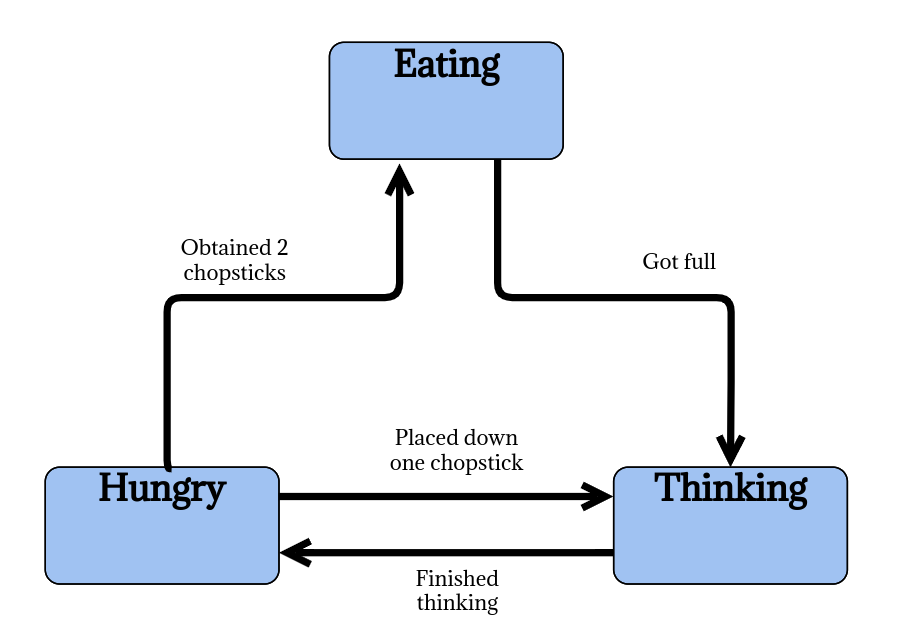
\includegraphics[scale=0.3]{images/livelock-state-diagram.png}
    \caption{State Diagram for Livelock}
\end{figure}

In the model with a central dining table, we had two types of components: the dining philosophers and the dining table.  We created five 
philosophers and one dining table in our Python file, and gave each philosopher a link to the dining table.  By doing so, we held all 
our chopsticks in one central location and made sure there were no duplicate copies of anything.  The philosophers would send message requests 
over their links if they needed to pick up a chopstick or put one back on the table.  The dining table received these events, and would 
let each philosopher know whether or not those chopsticks were actually available or not.  The information contained within each of those request 
events is detailed in the \texttt{requests.h} header file.  In addition, we have an illustration of this model generated by our simulation below.

\begin{figure}[H]
    \centering
    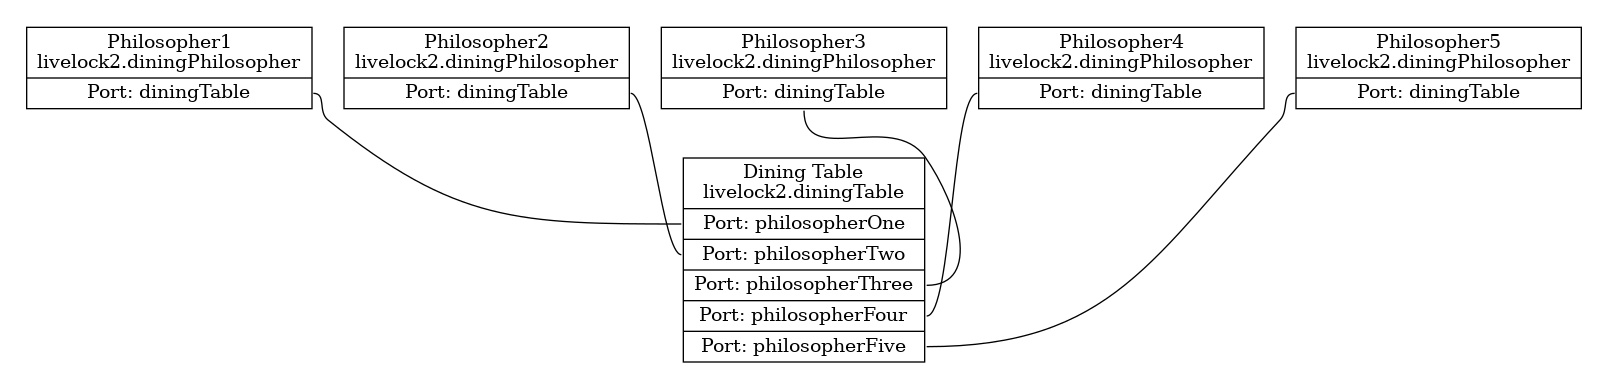
\includegraphics[scale=0.3]{images/livelock2.png}
    \caption{Visualization of Simulation Graph for Dining Table Example}
\end{figure}

In our other model, we replaced the central dining table component with individual chopsticks. Instead of each philosopher only having 
one link to the table, both philosophers and chopsticks had two links to keep track of.  Each philosopher had a link to both their left and 
right chopstick, and each chopstick had a link to their left and right philosopher.  In a similar fashion to the model described above, 
philosophers can take possession or place down their chopsticks by sending requests over their links.  The only difference here is that 
each chopstick only communicates with its adjacent philosophers as opposed to having one object managing the resources of the system. As before, we have an illustration of the model generated by our simulation below.

\begin{figure}[H]
    \centering
    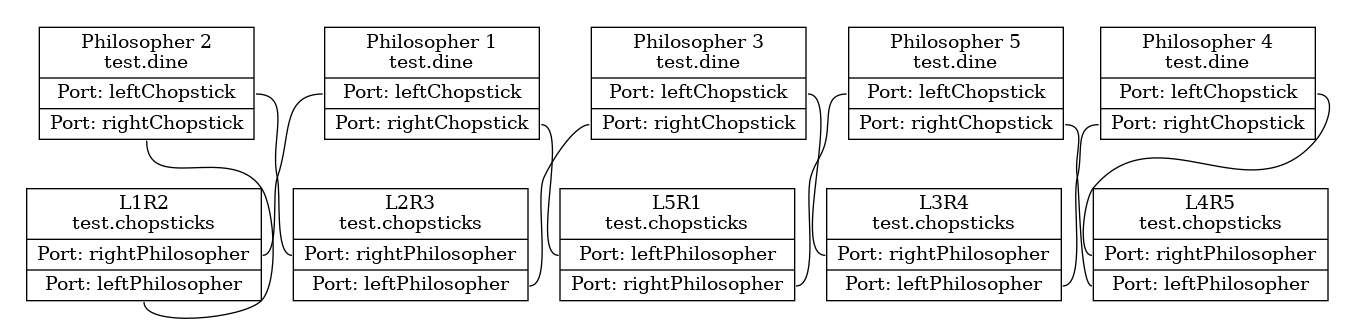
\includegraphics[scale=0.3]{images/test.png}
    \caption{Visualization of Simulation Graph for Chopstick Example}
\end{figure}

One other model we had included, though not directly relevant to this issue of livelock, was a model that simulates deadlock.  The 
only difference between livelock and deadlock in the dining philosopher’s problem is that the philosophers won’t check to see if they 
need to place a chopstick down if they’re only holding one.  Within SST, this is what our waiting clock does.  By removing the second clock, 
we force the philosophers into a deadlock scenario, where each only holds one chopstick and no one ever eats.  We can see a clearer distinction between the two models by looking at the state diagram for deadlock below.  Once we remove the transition from hungry to thinking, we don't have an interior loop within the state diagram.

\begin{figure}[H]
    \centering
    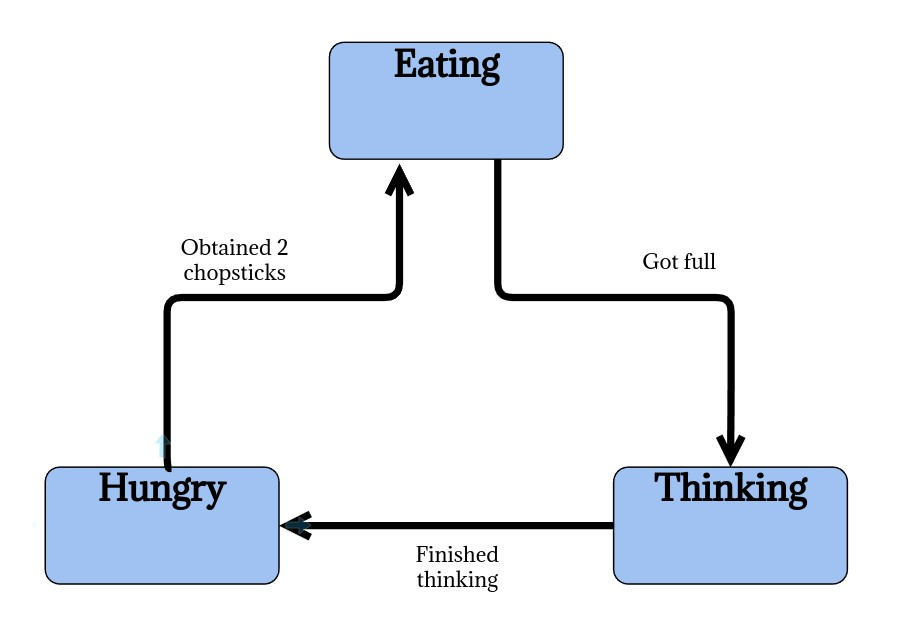
\includegraphics[scale=0.3]{images/deadlock-state-diagram.jpg}
    \caption{State Diagram for Deadlock}
\end{figure}

When comparing both of these models, both of them produce very similar results, however, the model with individual chopsticks seemed 
to take longer to update their status.  We can assume this would be due to the fact that there are double the amount of links in the 
chopstick model.  We believe that the benefit that the chopstick model gives us is that from a logical point of view, it makes more 
sense to view the chopstick as its own component, as opposed to a dining table, which isn't something discussed as heavily in the 
definition of the dining philosopher’s problem.  However, the benefit that the dining table model gives us is that it means we already 
have a central node in place that can double as a way to collect information from all the philosophers.  In addition, since this model 
only requires each component to have one link, it’d be easier to extend this model to have more philosophers or chopsticks. \newline

Lastly, an important thing to note about these models is that they were designed specifically with the idea in mind that there 
would be the same number of chopsticks and philosophers.  For example, the dining table keeps track of which philosophers would be 
allowed to access each chopstick. (eg. Chopstick “L5R1” is only accessible as Philosopher 1’s right chopstick, and Philosopher 5’s 
left chopstick).  The chopstick model also has a similar designation.  This would be important to keep in mind if you wanted to alter 
the simulation to have an uneven number of chopsticks to philosophers, where certain components weren’t predetermined to only be 
accessible to a specific subset of other components.  Generally speaking, the dining philosophers problem is designed to have an 
equal number of philosophers to chopsticks, but if you wanted to change the model in any way, this would be an important distinction.  

\section{Results} % conclusion/summary

% The result is ...
After we had established our models, we ran different sets of simulations on each set, observing when our philosophers actually 
experienced livelock.  The main thing that affected whether or not we experienced livelock was the changes we made to the timing 
parameters of the simulation.  Generally speaking, the more randomization you introduce into the timing, the less likely you are 
likely to experience livelock, with livelock being defined as the state in which none of the philosophers are ever able to enter 
their eating states.  In addition, \texttt{waitingDuration} should generally be less than or equal to \texttt{thinkingDuration} if you 
want to experience livelock.  In general, as long as each philosopher tries to grab the chopstick at the same time and puts them 
down at the same time, you are likely to enter a livelocked scenario. \newline

In terms of the metrics we coined in order to detect livelock, our current findings is that they are heavily reliant on the 
specific problem at hand.  For example, much of the work in this area tends to agree that livelock is dependent on an existence 
of some infinite loop that contains changing states, as well as the lack of progress in the system.  In addition to this, many 
sources tend to agree that the definition of progress, as well as the definition of infinite is something that is left up to the 
programmer to decide, as it varies per problem.  We can define those criteria in the dining philosopher's problem by looking towards 
how much time one spends switching between thinking and being hungry, and how often one eats. \newline

Taking this information, we decided to define our metrics in terms of the progress we made in the system.  We let our simulation run 
for an extended period of time defined by our parameters, and at that point check in on the status of each of our states: thinking, 
hungry, and eating.  From here, we wait for another period of time that we designated as our "window" so we could do \href{https://en.wikipedia.org/wiki/Time_series}{time series analysis}. As this window closes, we once 
again take note of each of our states, counting how many times we entered each one.  Once we have this data, we can first note whether or not we allowed the philosopher to eat at all.  
This tells us whether or not we made progress in our system.  After this, we can check the rate at which each philosopher switched from 
thinking to hungry.  We do this by measuring in our window the amount of switches that happened, and generating a percentage of time spent 
in each state based on what we expect.  In a livelock scenario, we would spend about half our time hungry, and half our time thinking, so 
we divide our window size by two.  This gives us a fraction of the actual number of switches into a certain state over the expected number of 
switches into a certain state.  The higher each percentage is, the more likely it is to be livelocked, especially if there was no progress 
made in this window.  In true livelock, our hungry boolean would show us that no one ate, and that each of our percentages show that the 
philosopher spent all their time in either the hungry or thinking state. \newline

To imagine these metrics a bit more clearly, suppose we have a window size of 100 cycles.  Within our simulation, we could enter any of our 3 states during this window. In a normal scenario, we could spend an approximately equal amount of time in each state (33 cycles eating, 33 cycles thinking, 34 cycles hungry), or an uneven distribution in each state (20 cycles hungry, 50 cycles thinking, 30 cycles eating), all depending on the parameters passed into the simulation.  However, if we enter a livelock state, we know we're only going to think or be hungry, and that we will constantly switch back and forth between these two states at an even rate defined by our clock.  Because of this, in our 100 cycle window, we would spend 50 cycles thinking, 50 cycles hungry, and 0 cycles eating.  Based off of this, we generate our percentages as discussed above, and our expected state count for each of the two states in livelock to be (window size/2).  In our example, at the end of the 100 cycle window, our uneven livelock distribution above would give us 60\% of the expected eating time spent actually eating (30 cycles eating/50 expected cycles eating).  Although we get 100\% of the expected time thinking (50 cycles thinking/50 expected cycles thinking), the fact that both values aren't at 100\% is an indication to us that this particular philosopher isn't livelocked within this window. \newline

In order to view this output in an actual simulation, we utilized a combination of SST output functionalities.  First off, if you want to see text updates of what happened in the simulation, you can look to the .txt output from the simulation.  Based on how detailed you want this output to be, you can select different verbosity levels in the Python file.  Level 1 gives livelock updates every window, level 2 lets you know when different components send or receive message requests, level 3 lets you know when a philosopher switches states, and level 4 gives general updates on the state of every component at every cycle.  In addition to this, the information regarding the livelock updates is also outputted to .csv files, where each philosopher gets their own file with a cycle indication, as well as the hungry boolean and our thinking and hungry percentages to be outputted as graphs. \newline

Above, we show an example of what these graphs would look like, and how we can induce livelock in the simulation.  The graph on the left shows one of our 5 philosophers once they entered livelock, while the one on the right shows a system that didn't experience livelock.  The red and blue lines represent the thinking state and hungry state percentages, and the yellow line marks the boolean of whether or not we've eaten in a certain window.  As you can see, when there's no livelock, we see a lot of flcuations in the amount of time spent thinking and hungry, and that our boolean tends to be false.  On the other hand, our livelock scenario shows that we spend all our time thinking and hungry, and that we never once eat.  Graphs for the rest of the philosophers in these 2 simulations can be found in the appendix.  The important thing to note is that the livelock scenario has equal ThinkingDurations for each philosopher, while the non-livelock scenario has randomized ThinkingDurations.  Generally speaking, if we see more flucuations in our graphs, or we observe that the philosopher has eaten, we can conclude that there isn't any livelock for that philosopher.  On the other hand, when we constantly flip between only two states and never eat, we are likely to be livelocked.

\begin{figure}%
    \centering
    \subfloat[\centering Philosopher 2 in a non livelock state]{{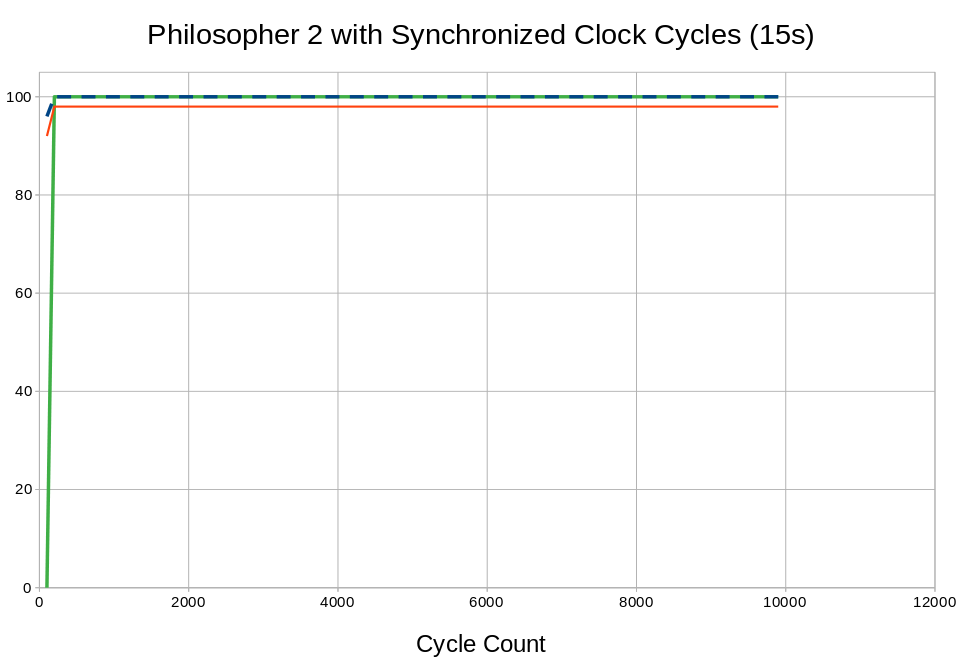
\includegraphics[width=7.5cm]{images/NonLivelockedPhilosopher.png} }}%
    \qquad
    \subfloat[\centering Philosopher 2 in a livelock state]{{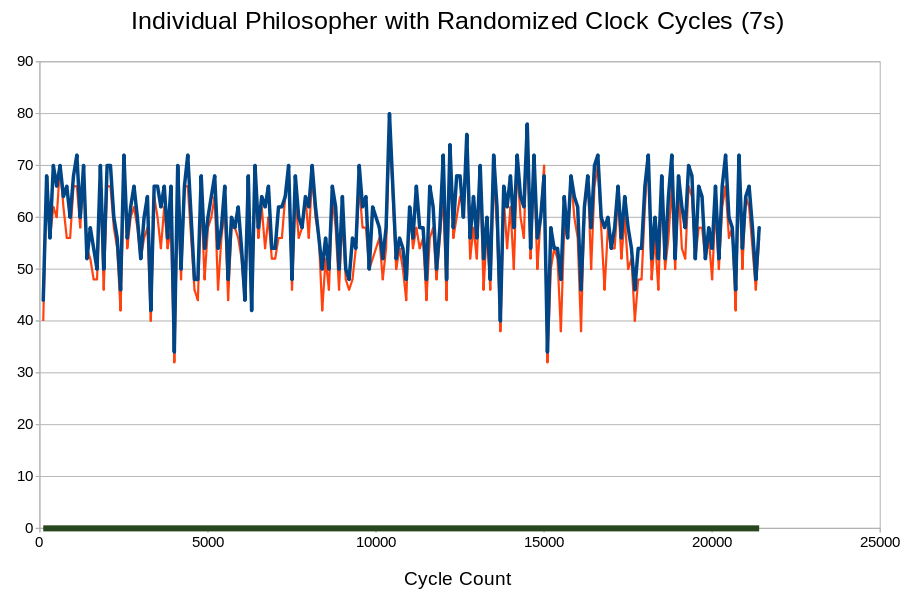
\includegraphics[width=7.5cm]{images/LivelockedPhilosopher.png}}}%
    \caption{Comparison of Different \texttt{ThinkingDurations} on One Philosopher}%
    \label{fig:example}%
\end{figure}


\section{Future Work} % areas that still need more research
The lack of concrete research in regards to both livelock as a whole, as well as the specifics of how to quantify livelock issues limited this project.  Many papers had differing definitions on what qualified as livelock, and these various definitions were sometimes hard to translate into useful information for distributed systems, such as what would be considered an infinite loop, or what was meant by progress in the system.  To further understand this problem, it would probably be most helpful to find more real examples of livelock (eg. not the hallway problem), so that we can come up with metrics that are applicable to a wider set of systems.  In addition, we could potentially alter the simulation to observe a wider set of problems.  For example, our current simulation hard-codes which philosophers can use which chopsticks, as well as the number of both chopsticks and philosophers.  It may be helpful to alter this simulation to vary who can grab which resource, which would potentially allow us to create situations of partial livelock.  It would also allow us to scale the simulation up, and observe what happens if there were, for example, 500 philosophers instead of just 5.  Lastly, we could also attempt to inject errors into the links to see if this would affect anything.  For example, if one link went down for 20 cycles, we could observe how the affected philosophers would try to communicate with others, as well as if they'd be able to switch back to their original link after it was working properly again.  Encouraging problems like these would both help us model distributed systems in a more realistic manner, and allow us to see if it would change the way in which livelock occured.  While we can conclude that we have livelock in the simulations provided above, finding ways to generalize the process in which we found livelock would be useful  (eg. a more general definition of progress, or clearer examples of states that don't only apply to dining philosophers). 

\section{Appendix}
\begin{figure}[H]
    \centering
    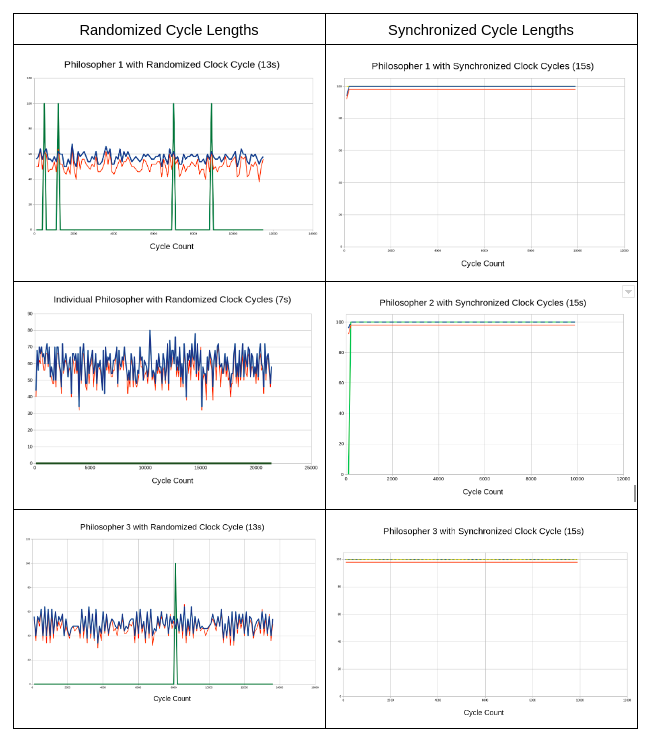
\includegraphics[scale=0.70]{images/NewGraphs1.png}
\end{figure}
\begin{figure}[H]
    \centering
    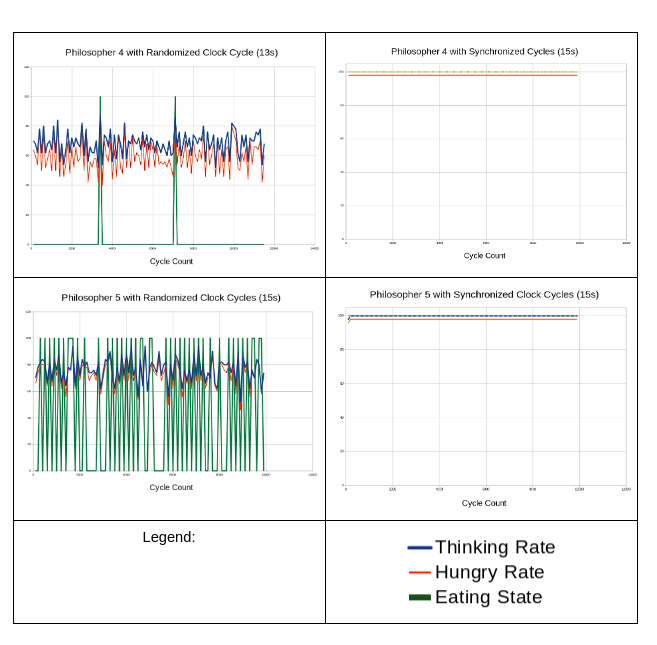
\includegraphics[scale=0.7]{images/NewGraphs2.png}
\end{figure}

\begin{thebibliography}{9}
\bibitem{texbook}
Donald E. Knuth (1986) \emph{The \TeX{} Book}, Addison-Wesley Professional.

\bibitem{lamport94}
Leslie Lamport (1994) \emph{\LaTeX: a document preparation system}, Addison
Wesley, Massachusetts, 2nd ed.

\bibitem{k.tai}
Kuo-Chung Tai (1994) Definitions and Detection of Deadlock, Livelock, and Starvation in Concurrent Programs, IEEE Computer Society

\bibitem{a.ho}
Alex Ho (2005) On Deadlock, Livelock, and Forward Progress

\bibitem{j.fiedor}
Jan Fiedor (2010) A Uniform Classification of Common Concurrency Errors

\end{thebibliography}

\end{document}
